\documentclass[smaller]{beamer}
\usetheme[english]{Berlin}
\usepackage{ngerman}
\useoutertheme{infolines}
\beamertemplatenavigationsymbolsempty
\usepackage{pgfplots,tikz,subfigure}
\usepackage{amsmath,amsthm}
\usepackage{hyperref,graphics,graphicx,color,algorithm,algorithmic,enumerate}
\usepackage{mymacros,wrapfig,relsize}
\usepackage{pict2e}
\usepackage[utf8x]{inputenc}

\newcommand{\ri}{\mathrm{i}}
\newcommand{\T}{\mathsf{T}}
\renewcommand{\H}{\mathsf{H}}
\newcommand{\eps}{\varepsilon}
\newcommand{\To}{\rightarrow}
\newcommand{\sddots}{\scalebox{0.6}{$\ddots$}}
\usepackage[pdf]{pstricks}
\usepackage{sansmathfonts}
\usepackage{eurosym}
%\usepackage{arev}
%\renewcommand\familydefault{\sfdefault}

\DeclareMathOperator{\loc}{loc}
\DeclareMathOperator{\rank}{rank}
\DeclareMathOperator{\RE}{Re}
\DeclareMathOperator{\IM}{Im}
\DeclareMathOperator{\In}{In}
\DeclareMathOperator{\im}{im}
\DeclareMathOperator{\Gl}{Gl}
\DeclareMathOperator{\spa}{span}
\DeclareMathOperator{\ext}{{ext}}
\DeclareMathOperator{\ind}{ind}
\DeclareMathOperator{\normalrank}{normalrank}
\DeclareMathOperator{\essup}{ess\,sup}
\DeclareMathOperator{\vect}{vec}

\newcommand{\re}{\mathrm{e}}
\newcommand{\ddt}{\tfrac{\mathrm{d}}{\mathrm{d}t}}
\newcommand{\sys}[4]{\left[\begin{array}{c|c} #1 & #2 \\ \hline #3 & #4 \end{array}\right]}

\renewcommand{\tilde}{\widetilde}
\renewcommand{\hat}{\widehat}


\title[]{Optimierung f\"ur Studierende der Informatik}
\subtitle{-- 6. Vorlesung --}
\author[Matthias Voigt]{\textbf{Matthias Voigt$^{1,2}$}}
\institute[]{
\begin{columns}
%\begin{center}
\column{0.45\textwidth}{\centering {$^1$Universit\"at Hamburg \\ Fachbereich Mathematik \\ Hamburg \\ }}
\column{0.45\textwidth}{\centering {$^2$Technische Universit\"at Berlin \\ Institut f\"ur Mathematik \\ Berlin  \\}}
%\end{center}
\end{columns}
}
\date[]{Universit\"at Hamburg
\begin{columns}
\column{0.45\textwidth}{\centering 
\includegraphics[width = 1.2\textwidth]{uhh-logo.png}\\}
\end{columns}
}

\definecolor{tucgreen}{rgb}{0.0,0.5,0.27}
\definecolor{tucred}{rgb}{0.75,0,0}
\definecolor{tucorange}{rgb}{1.0,.5625,0}
\definecolor{mpired}{HTML}{990000}
\definecolor{mpigreen}{HTML}{5C871D}
\definecolor{mpiblue}{HTML}{006AA9}
\definecolor{mpibg1}{HTML}{5D8B8A}
\definecolor{mpibg2}{HTML}{BFDFDE}
\definecolor{mpibg3}{HTML}{A7C1C0}
\definecolor{mpibg4}{HTML}{7DA9A8}
\definecolor{mpigrey}{rgb}{0.9294,0.9294,0.8784}

\begin{document}

\maketitle

\begin{frame}
\frametitle{Eine Iteration im revidierten Simplexverfahren}
\begin{enumerate}[a)]
\item\textbf{1. Schritt:} Man löse das Gleichungssystem $y^TB = c_B^T$.

\item\textbf{2. Schritt:} Wahl der Eingangsspalte; es kommt jede Spalte $a$ von $A_N$ infrage, für die $y^Ta$ kleiner ist als die entsprechende Komponente von $c_N^T$. Falls es keine solche Spalte gibt, ist die aktuelle Lösung optimal.

\item\textbf{3. Schritt:} Man löse das Gleichungssystem $Bd=a$.

\item\textbf{4. Schritt:} Man finde das größte $t \geq 0$, für das $x_B^*-td \geq 0$ gilt. Falls es kein solches $t$ gibt, ist das Problem unbeschränkt; andernfalls ist mindestens eine Komponente von $x_B^*-td$ gleich Null und eine zugehörige Variable verlässt die Basis.
\item\textbf{5. Schritt:} Man setze den Wert der Eingangsvariablen auf $t$ (für das größtmögliche $t$ wie im 4. Schritt) und ersetze in $x_B^*$ die Werte der übrigen Basisvariablen durch $x_B^* - td$. Außerdem ersetze man in $B$ die Ausgangsspalte durch die Eingangsspalte. Beim Update von $x_B^*$ und $B$ beachte man die zuvor beschriebene Regel.
\end{enumerate}
\end{frame}

\begin{frame}
 \frametitle{Beispiel}
 Wir greifen unser erstes Beispiel zur Standardsimplexmethode aus Vorlesung 1 wieder auf und wollen es nun mit dem revidierten Simplexverfahren lösen. Dieses Beispiel lautet wie folgt:

\begin{align*}
\begin{alignedat}{5}
& \text{maximiere } & 5x_1 &\ + &\ 4x_2 &\ + &\ 3x_3 & & \\
& \rlap{unter den Nebenbedingungen} & & & & & & & \\
&& 2x_1 &\ + &\ 3x_2 &\ + &\  x_3 &\ \leq &\  5,\ \\
&& 4x_1 &\ + &\  x_2 &\ + &\ 2x_3 &\ \leq &\ 11,\ \\
&& 3x_1 &\ + &\ 4x_2 &\ + &\ 2x_3 &\ \leq &\  8,\ \\
&& & & & & \llap{$x_1, x_2, x_3$} &\ \geq &\  0.\
\end{alignedat}
\end{align*}
\end{frame}

\begin{frame}
 \frametitle{Die Problemdaten}
 Die \structure{Problemdaten} für unser Beispiel sind gegeben durch\footnote{Es ist zweckmäßig und sehr zu empfehlen, sowohl bei $A$ als auch bei $c^T$ eine \structure{Kopfzeile} der Form $x_1,\ldots,x_n$ hinzuzufügen. Schreibt man $A$ und $c^T$ genau untereinander, so genügt es, die Kopfzeile nur bei $A$ anzugeben.}
\begin{align*}
A &= \bordermatrix{ & x_1 & x_2 & x_3 & x_4 & x_5 & x_6 \cr & 2 & 3 & 1 & 1 & 0 & 0 \cr & 4 & 1 & 2 & 0 & 1 & 0 \cr & 3 & 4 & 2 & 0 & 0 & 1},\quad
b = \begin{pmatrix} 5 \\ 11 \\ 8 \end{pmatrix} \quad \text{und} \\ 
c^T &= \bordermatrix{ & x_1 & x_2 & x_3 & x_4 & x_5 & x_6 \cr & 5 & 4 & 3 & 0 & 0 & 0}.
\end{align*}
\end{frame}

\begin{frame}
 \frametitle{Initialisierung}
 Das Verfahren startet mit 
\[
x_B^* = \begin{pmatrix} x_4^* \\ x_5^* \\ x_6^* \end{pmatrix} = \begin{pmatrix} 5 \\ 11 \\ 8 \end{pmatrix} \quad \text{und} \quad
B = \bordermatrix{ & x_4 & x_5 & x_6 \cr & 1 & 0 & 0 \cr & 0 & 1 & 0 \cr & 0 & 0 & 1}.
\]

Auch bei $B$ wurde eine \alert{Kopfzeile} hinzugefügt, die angibt, wie sich Basisvariablen und Spalten entsprechen. Dies dient der Übersichtlichkeit. \alert{Bei der Basismatrix $B$ ist das Hinzufügen der Kopfzeile besonders wichtig}, da die Spalten von $B$ nicht immer in derselben Reihenfolge wie in $A$ vorkommen. \\ \vspace*{0.2cm}

Auch bei der Matrix $A_N$ fügen wir im Folgenden eine Kopfzeile hinzu. 
\end{frame}

\begin{frame}
 \frametitle{1. Schritt der 1. Iteration}
 {\textbf{1. Schritt:}} Das Gleichungssystem $y^TB = c_B^T$ lautet
\begin{align*}
\begin{alignedat}{4}
 y_1 &\ + &\ 0y_2 &\ + &\ 0y_3 &\ = &\ 0,\ \\
0y_1 &\ + &\  y_2 &\ + &\ 0y_3 &\ = &\ 0,\ \\
0y_1 &\ + &\ 0y_2 &\ + &\  y_3 &\ = &\ 0.\ 
\end{alignedat}
\end{align*}

Lösung: $y^T = (y_1,y_2,y_3) = (0,0,0)$.
\end{frame}

\begin{frame}
 \frametitle{2. Schritt der 1. Iteration}
 {\textbf{2. Schritt:}} Es gilt $A_N = \bordermatrix{ & x_1 & x_2 & x_3 \cr & 2 & 3 & 1 \cr & 4 & 1 & 2 \cr & 3 & 4 & 2}$; \\ \vspace*{0.2cm}
 
 für alle Spalten $a$ von $A_N$ gilt $y^Ta = 0$ und die Komponenten von $c_N^T$ lauten 5, 4 und 3. Es kommen also \alert{alle Spalten} von $A_N$ als Eingangsspalte $a$ infrage;\\ \vspace*{0.2cm}
 
 wir wählen $a = \begin{pmatrix} 2 \\ 4 \\ 3 \end{pmatrix}$.\\ \vspace*{0.2cm}
 
 Dies entspricht der Regel des größten Koeffizienten. Mit der Wahl der Eingangsspalte $a$ liegt auch die Eingangsvariable fest: In unserem Fall ist dies $x_1$.
\end{frame}

\begin{frame}
 \frametitle{3. Schritt der 1. Iteration}
 {\textbf{3. Schritt:}} Das Gleichungssystem $Bd=a$ lautet
\begin{align*}
\begin{alignedat}{4}
 d_1 &\ + &\ 0d_2 &\ + &\ 0d_3 &\ = &\ 2,\ \\
0d_1 &\ + &\  d_2 &\ + &\ 0d_3 &\ = &\ 4,\ \\
0d_1 &\ + &\ 0d_2 &\ + &\  d_3 &\ = &\ 3.\ 
\end{alignedat}
\end{align*}

Lösung: $d = \begin{pmatrix} 2 \\ 4 \\ 3 \end{pmatrix}$.
 
\end{frame}

\begin{frame}
 \frametitle{4. Schritt der 1. Iteration}
{\textbf{4. Schritt:}} Es ist das größte $t \geq 0$ zu finden, für das gilt:
\[
\begin{pmatrix} 5 \\ 11 \\ 8 \end{pmatrix} - t \begin{pmatrix} 2 \\ 4 \\ 3 \end{pmatrix} \geq \begin{pmatrix} 0 \\ 0 \\ 0 \end{pmatrix}.
\]

Für $t$ soll demnach
\begin{align*}
\begin{alignedat}{3}
 5 &\ - &\ 2t &\ \geq &\ 0, \\
11 &\ - &\ 4t &\ \geq &\ 0, \\
 8 &\ - &\ 3t &\ \geq &\ 0\
\end{alignedat}
\end{align*}

gelten. Das größte $t$, das dies erfüllt, ist $t=2.5$. Für diese Wahl von $t$ gilt
\[
x_B^* - td = \begin{pmatrix} 5-2t \\ 11-4t \\ 8-3t \end{pmatrix} = \begin{pmatrix} 0 \\ 1 \\ 0.5 \end{pmatrix}.
\]

Wegen $x_B^* = \begin{pmatrix} x_4^* \\ x_5^* \\ x_6^* \end{pmatrix}$ erhält man also $x_4$ als Ausgangsvariable.
\end{frame}

\begin{frame}
 \frametitle{5. Schritt in der 1. Iteration}
 \textbf{5. Schritt (Update von $x_B^*$ und $B$):}
Man erhält
\[
x_B^* = \begin{pmatrix} x_1^* \\ x_5^* \\ x_6^* \end{pmatrix} = \begin{pmatrix} 2.5 \\ 1 \\ 0.5 \end{pmatrix} \quad \text{und} \quad
B = \bordermatrix{ & x_1 & x_5 & x_6 \cr & 2 & 0 & 0 \cr & 4 & 1 & 0 \cr & 3 & 0 & 1 }. 
\]

Mit dem neuen Vektor $x_B^*$ und der neuen Basismatrix geht es nun in die nächste Runde.
\end{frame}

\begin{frame}
 \frametitle{2. Iteration}
 Die 2. Iteration verläuft ähnlich wie dir erste. Die Details der 2. Iteration werden in der Vorlesung nicht vorgetragen: Sie finden sie im Skript auf den Seiten 102 und 103. \\ \vspace*{0.2cm}

 \textbf{Empfehlung:} Arbeiten Sie die Details zur 2. Iteration zuhause selbstständig durch. \\ \vspace*{0.2cm} 

\alert{Hier ist das Ergebnis der 2. Iteration:} Als Update von $x_B^*$ und $B$ erhält man
\[
x_B^* = \begin{pmatrix} x_1^* \\ x_5^* \\ x_3^* \end{pmatrix} = \begin{pmatrix} 2 \\ 1 \\ 1 \end{pmatrix} \quad \text{und} \quad
B = \bordermatrix{ & x_1 & x_5 & x_3 \cr & 2 & 0 & 1 \cr & 4 & 1 & 2 \cr & 3 & 0 & 2 }.
\]

Mit dem neuen Vektor $x_B^*$ und der neuen Basismatrix geht es nun in die nächste Runde.
\end{frame}

\begin{frame}
 \frametitle{1. Schritt der 3. Iteration}
 {\textbf{1. Schritt:}} Das zu lösende Gleichungssystem lautet\footnote{Man beachte: Zu lösen ist $y^TB = c_B^T$, wobei die Spalten von $B$ in der Reihenfolge auftreten, die der Kopfzeile $x_1,x_5,x_3$ entspricht. \alert{Diese Reihenfolge ist auch für die rechten Seiten des Gleichungssystems einzuhalten}. Dementsprechend gilt $c_B^T = (5,0,3)$.}
\begin{align*}
\begin{alignedat}{4}
2y_1 &\ + &\ 4y_2 &\ + &\ 3y_3 &\ = &\ 5,\ \\
     &\   &\  y_2 &\   &\      &\ = &\ 0,\ \\
 y_1 &\ + &\ 2y_2 &\ + &\ 2y_3 &\ = &\ 3.\ 
\end{alignedat}
\end{align*}

Lösung: $y^T = (y_1,y_2,y_3) = (1,0,1)$.
\end{frame}

\begin{frame}
 \frametitle{2. Schritt der 3. Iteration}
\textbf{2. Schritt:} Es gilt $A_N = \bordermatrix{ & x_2 & x_4 & x_6 \cr & 3 & 1 & 0 \cr & 1 & 0 & 0 \cr & 4 & 0 & 1 }$. \\ \vspace*{0.2cm}

Für die Spalten $a$ von $A_N$ ergeben sich die folgenden Werte von $y^Ta$: 7, 1, 1. Als dazugehörige Einträge von $c_N^T$ haben wir 4, 0, 0. \alert{Es folgt, dass die aktuelle Lösung optimal ist.} \\ \vspace*{0.2cm}

Als \alert{optimale Basislösung} hat sich ergeben:
\[
x_1^*=2,\quad
x_2^*=0,\quad
x_3^*=1,\quad
x_4^*=0,\quad
x_5^*=1,\quad
x_6^*=0.
\]

Als \alert{optimalen Zielfunktionswert} erhält man $z=13$.
\end{frame}

\begin{frame}
 \frametitle{Standardmethode vs. revidiertes Verfahren}
 Für beide Varianten gilt: \alert{In jeder Iteration wird eine zulässige Basislösung durch eine in der Regel andere zulässige Basislösung ersetzt}. Oder, in geometrischer Terminologie ausgedrückt:
\begin{quote} 
\alert{Man bewegt sich auf dem Rand des zulässigen Bereichs ({\glqq}längs einer Kante{\grqq}) von einer Ecke zur nächsten.}
\end{quote}

Die \alert{Details} sind jedoch sehr unterschiedlich:
\end{frame}

\begin{frame}
 \frametitle{Standardmethode vs. revidiertes Verfahren}
 \begin{itemize}
\item Im Standardverfahren arbeitet man mit \alert{Tableaus}, in denen sich die aktuelle zulässige Basislösung unmittelbar ablesen lässt; \alert{in jeder Iteration wird das neue Tableau direkt aus dem vorhergehenden Tableau berechnet}.
\item Im Gegensatz dazu berechnet man in jeder Iteration des revidierten Simplexverfahrens die neue zulässige Basislösung direkt \alert{aus den Problemdaten}, wobei zwei lineare Gleichungssysteme zu lösen sind. \alert{Man berechnet dabei nicht das komplette Tableau, sondern nur den Teil, den man wirklich benötigt!}
\end{itemize}

Beide Varianten haben \alert{Vor- und Nachteile:} Diese werden im Buch von Chvátal ausführlich beschrieben und diskutiert; vgl. auch K. Neumann, M. Morlock: \textit{Operations Research} (Hanser Verlag), wo ebenfalls die ``pros and cons'' der beiden Varianten diskutiert werden. Hier soll nur ein Punkt etwas genauer besprochen werden.
\end{frame}

\begin{frame}
 \frametitle{Sehr große und schwach besetzte Probleme}
In der \alert{Praxis} hat man es meist mit \alert{sehr großen Problemen} zu tun: Probleme mit mehr als 100000 Variablen und beispielsweise $m=10000$ Gleichungen (Nebenbedingungen) sind keine Seltenheit. Häufig handelt es sich dabei um \alert{Probleme, bei denen die meisten Koeffizienten $a_{ij}$ gleich Null sind}. Man spricht dann von \structure{schwach besetzten Problemen} und \structure{schwach besetzten Matrizen}. \\ \vspace*{0.2cm} 

Typische Größen\-ord\-nungen: $n=100000$ Variablen, $m=10000$ Gleichungen, aber niemals mehr als 10 Einträge in jeder Spalte der Matrix $(a_{ij})$, die ungleich Null sind.
\end{frame}

\begin{frame}
 \frametitle{Sehr große und schwach besetzte Probleme}
Zur Behandlung von LP-Problemen mit schwach besetzten Matrizen gibt es ausgefeilte Methoden (vgl. etwa Chvátal, Kapitel 7 und 24). Man kann sagen: \alert{Sind LP-Probleme sehr groß, so werden sie überhaupt nur dadurch für die Behandlung in einem Computer zugänglich, dass es sich um schwach besetzte Probleme handelt}. \\ \vspace*{0.2cm}

Beispielsweise müssen die vielen Nullen nicht gespeichert werden, sondern man speichert nur, an welchen Stellen Einträge ungleich Null stehen -- und natürlich die Werte dieser Einträge.
\end{frame}

\begin{frame}
 \frametitle{Sehr große und schwach besetzte Problem}
 Nach diesen Bemerkungen wird klar, weshalb in der Praxis, wenn es um sehr große, schwach besetzte Matrizen geht, \alert{die revidierte Simplexmethode vorzuziehen ist:}
\begin{itemize}
	\item Beim \alert{Standardsimplexverfahren} kann aus dem Anfangstableau nach wenigen Iterationen ein {\glqq}stark besetztes Tableau{\grqq} werden, d.h. ein Tableau, in dem viele Einträge ungleich Null sind. Diese Einträge müssen alle gespeichert werden, d.h., der Vorteil, den man am Anfang durch das Vorliegen eines schwach besetzten Problems hat, ist {\glqq}futsch{\grqq}.
	\item Dergleichen kann beim \alert{revidierten Verfahren} nicht passieren, da man in jeder Iteration mit den Spalten der schwach besetzten Matrix $A$ arbeitet und nicht mit einem völlig neuen Tableau, das in der Regel nicht mehr schwach besetzt ist.
\end{itemize}
\end{frame}

\begin{frame}
 \frametitle{Ein weiterer Grund}
Wir haben einen der Gründe angesprochen, weshalb praxistaugliche Softwarepakete auf dem revidierten Simplexverfahren basieren  und nicht auf dem Standardverfahren. \\ \vspace*{0.2cm}

Hier noch ein anderer Grund: \alert{Häufig ist die Anzahl $n$ der Variablen wesentlich größer als $m$} (= Anzahl der Nebenbedingungen ohne die Nichtnegativitätsbedingungen). Daher kann es ein großer Vorteil sein, dass man im revidierten Verfahren im Wesentlichen mit der Basismatrix $B$ arbeitet. (Man beachte: $B$ ist eine $m \times m$ - Matrix, während in einem Tableau $n$ Spalten vorkommen.) \\ \vspace*{0.2cm}

\alert{Für die Bearbeitung kleinerer Probleme per Hand sind beide Varianten -- die Standardmethode und das revidierte Verfahren -- sehr gut geeignet}.
\end{frame}

\begin{frame}
 \frametitle{Flussnetzwerke}
 Wir betrachten gerichtete Graphen, in denen jede Kante eine {\glqq}Kapazität{\grqq} besitzt. Je nach Anwendungszusammenhang können diese Kapazitäten eine unterschiedliche Bedeutung haben. \\ \vspace*{0.2cm} 
 
 In jedem Fall geht es jedoch um \alert{obere Schranken:} Beispielsweise besitzen Stromleitungen eine Maximalbelastung, durch eine Wasserleitung kann nur eine bestimmte Menge Wasser fließen oder auf einer Bahnstrecke kann nur eine gewisse Menge eines bestimmten Guts transportiert werden. \\ \vspace*{0.2cm}
 
 Zur Modellierung derartiger Situationen verwendet man sogenannte \structure{Flussnetzwerke} (kurz: \structure{Netzwerke}). Von grundlegender Bedeutung sind in diesem Zusammenhang \structure{gerichtete Graphen} (kurz: \structure{Digraphen}). Wir geben im Folgenden genaue Definitionen der erwähnten Begriffe. 
\end{frame}

\begin{frame}
 \frametitle{Grundlegende Definitionen}
\textbf{Definition:} 
\begin{itemize}
\item Es sei $G=(V,E)$ ein \structure{schlingenloser Digraph}, d.h., $V$ ist eine endliche Menge, deren Elemente \structure{Knoten} genannt werden, und $E$ ist eine Teilmenge von $V \times V$, die nur Paare $(a,b)$ aus $V \times V$ enthält, für die $a \neq b$ gilt. Die Elemente von $E$ heißen \structure{(gerichtete) Kanten}.

\item Außerdem sei $c: E \rightarrow \N \cup \bigl\{ 0 \bigr\}$ eine Abbildung, die jeder Kante $e \in E$ eine nichtnegative ganze Zahl $c(e)$ zuordnet, welche wir die \structure{Kapazität} von $e$ nennen.

\item Schließlich seien $s$ und $t$ zwei verschiedene Knoten von $G$, für die gilt: \alert{Zu $s$ führen keine Kanten hin und von $t$ führen keine Kanten weg.} 

\item Darüber hinaus wollen wir voraussetzen, dass es in $G$ \alert{keine isolierten Knoten} gibt, d.h., für jeden Knoten $v$ soll es mindestens eine Kante geben, die zu $v$ hin oder von $v$ weg führt.

\item Unter diesen Voraussetzungen nennen wir $N=(G,c,s,t)$ \structure{ein Flussnetzwerk} mit \structure{Quelle} $s$ und \structure{Senke} $t$ (kurz: \structure{Netzwerk}).
\end{itemize}
\end{frame}

\begin{frame}
 \frametitle{Beispiel}
 \textbf{Ein Beispiel:}
 \begin{center}
  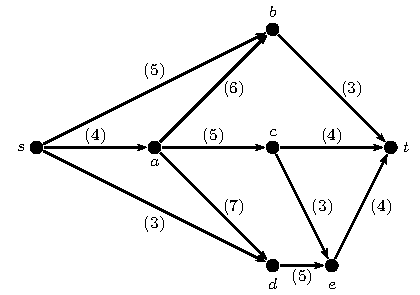
\includegraphics{fig7.pdf}
 \end{center}
Die eingeklammerten Zahlen bezeichnen die \alert{Kapazitäten} der Kanten.
\end{frame}

\begin{frame}
\frametitle{Flüsse durch Kanten}
Wir wollen uns nun für ein gegebenes Netzwerk zusätzlich vorstellen, dass in jeder Kante $e=(v,w)$ ein {\glqq}Fluss{\grqq} von $v$ nach $w$ vorliegt: Beispielsweise kann man sich die \alert{Kanten als Wasserleitungen} denken; oder man kann sich die Kanten $e=(v,w)$ \alert{als Straßen} vorstellen, auf denen irgendeine Ware von $v$ nach $w$ transportiert wird. Durch $f(e) \in \R$ soll die Stärke des Flusses von $v$ nach $w$ modelliert werden. \\ \vspace*{0.2cm}

Wir werden im Folgenden nur dann von einem Fluss auf dem Netzwerk $N$ sprechen, wenn für alle Kanten $e \in E$ gilt:
\[
0 \leq f(e) \leq c(e).
\]

Mit anderen Worten: $f(e)$ soll immer nichtnegativ sein und $f(e)$ soll die Kapazität $c(e)$ niemals über\-schrei\-ten. Außerdem soll eine \structure{Erhaltungsregel} für alle Knoten $v \neq s,t$ gelten: \alert{Es soll aus $v$ ebenso viel herausfließen, wie in $v$ hineinfließt}. \\ \vspace*{0.2cm}

Bevor wir nun all dies in einer Definition zusammenfassen, führen wir einige Schreibweisen ein.
\end{frame}

\begin{frame}
 \frametitle{Einige Schreibweisen}
 Gegeben sei ein Netzwerk $N=(G,c,s,t)$ mit $G=(V,E)$. Sind $X$ und $Y$ Teilmengen von $V$, so bezeichnen wir mit
\[
\big(X,Y\big)
\]
die Menge aller Kanten $(v,w) \in E$, für die $v \in X$ und $w \in Y$ gilt. Dasselbe in Mengenschreibweise:
\[
\big(X,Y\big) = \Big\{ (v,w) \in E : v \in X \text{ und } w \in Y \Big\}.
\]

Mit anderen Worten: \alert{$(X,Y)$ bezeichnet die Menge aller Kanten von $E$, die von $X$ nach $Y$ zeigen}.
\end{frame}

\begin{frame}
 \frametitle{Einige Schreibweisen (Fortsetzung)}
 Für eine Teilmenge $X$ von $V$ bezeichnen wir mit $\overline{X}$ das \structure{Komplement} von $X$ in $V$, d.h.,
\[
\overline{X} = V \setminus X.
\]

$\overline{X}$ ist also die Menge der Knoten aus $V$, die nicht in $X$ liegen, und $(X, \overline{X})$ ist die Menge der Kanten, die von $X$ nach $\overline{X}$ zeigen.

\begin{center}
 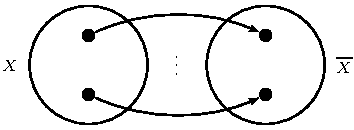
\includegraphics{fig8.pdf}
\end{center}

\end{frame}

\begin{frame}
 \frametitle{Einige Schreibweisen (Fortsetzung)}
 Es sei nun $f: E \rightarrow \R$ eine Funktion; $f$ ordnet also jeder Kante $e \in E$ eine reelle Zahl $f(e)$ zu. Dann definieren wir
\[
f(X,\overline{X}) := \sum\limits_{e \in (X,\overline{X})}{f(e)}.
\]

Um $f(X,\overline{X})$ zu berechnen, sind also alle Kanten $e \in E$ zu betrachten, die von $X$ nach $\overline{X}$ zeigen; für diese Kanten sind die Werte $f(e)$ aufzusummieren. \\ \vspace*{0.2cm}

Als \alert{Abkürzung} schreiben wir auch
\[
f^+(X) := f(X,\overline{X})
\]
sowie
\[
f^-(X) := f(\overline{X},X).
\]

Gilt $X = \bigl\{ v \bigr\}$, d.h., $X$ enthält nur den Knoten $v$, so schreiben wir anstelle von $f^+\left(\big\{ v \big\}\right)$ und $f^-\left(\big\{ v \big\}\right)$ auch einfach 
\[
f^+(v) \quad \text{und} \quad f^-(v).
\] 
\end{frame}

\begin{frame}
 \frametitle{Beispiel}
 \textbf{Beispiel:} Es sollen, wie in der folgenden Zeichnung dargestellt, fünf Kanten an $v$ stoßen.
 \begin{center}
  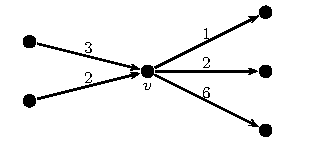
\includegraphics{fig9.pdf}
 \end{center}
Die Zahlen geben die Werte von $f$ an. Dann gilt
\[
f^-(v) = 3+2 = 5
\]
und
\[
f^+(v) = 1+2+6 = 9.
\]
\end{frame}

\begin{frame}
 \frametitle{Eine zentrale Definition}
 \textbf{Definition:} Gegeben sei ein Netzwerk $N=(G,c,s,t)$ mit $G=(V,E)$. Eine Abbildung
\[
f: E \rightarrow \R
\]

heißt ein \structure{Fluss} auf $N$, wenn $f$ den beiden folgenden Bedingungen genügt:
\begin{enumerate}[1)]
\item $0 \leq f(e) \leq c(e)$ für alle $e \in E$;
\item $f^-(v) = f^+(v)$ für alle Knoten $v \neq s,t$.
\end{enumerate}

Die Bedingung 2) bedeutet, dass für alle Knoten $v \neq s,t$ gilt\footnote{Knoten $v \in V$ mit $v\neq s,t$ nennt man auch \structure{innere Knoten} des Netzwerks $N$.}: \alert{Aus $v$ fließt ebenso viel hinaus, wie hineinfließt}.
\end{frame}

\begin{frame}
 \frametitle{Beispiel}
 \textbf{Beispiel}. Für das Netzwerk auf Folie 22 sei $f$ gegeben durch:
\[
\begin{array}{c|c}
(x,y) & f(x,y) \\ \hline\hline
(s,a) & 4 \\
(s,b) & 1 \\
(s,d) & 2 \\
(a,b) & 1 \\
(a,c) & 2 \\
(a,d) & 1 \\
(c,e) & 1 \\
(d,e) & 3 \\
(b,t) & 2 \\
(c,t) & 1 \\
(e,t) & 4
\end{array}
\]

Trägt man diese Werte in die zugehörige Zeichnung ein, so erkennt man sofort, \alert{dass 1) und 2) erfüllt sind, dass also ein Fluss vorliegt:}
\end{frame}

\begin{frame}
 \frametitle{Beispiel}
 \begin{center}
  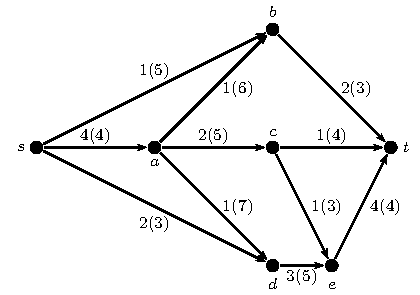
\includegraphics{fig10.pdf}
 \end{center}
%  Gilt $e = (v,w)$ für eine Kante $e \in E$, so nennen wir $v$ den \textit{Anfangsknoten}\index{Anfangsknoten einer Kante}\index{Kante!Anfangsknoten einer} von $e$ und $w$ ist der \textit{Endknoten}\index{Endknoten einer Kante}\index{Kante!Endknoten einer} von $e$. \\ \vspace*{0.2cm}

 Da an den inneren Knoten $v \neq s,t$ die Erhaltungsregel 2) gilt, ist es \alert{plausibel}, dass aus $s$ ebenso viel wegfließt, wie in $t$ ankommt: Dies ist der Inhalt der folgende Feststellung.
\end{frame}

\begin{frame}
 \frametitle{Der Wert eines Flusses}
  \textbf{Feststellung 1:}
  \[
   f^+(s) = f^-(t).
  \]
  
 \textbf{Definition:}
 Den aufgrund von Feststellung 1 gemeinsamen Wert von $f^+(s)$ und $f^-(t)$ nennt man den \structure{Wert des Flusses $f$} (Bezeichnung: $w(f)$). Man definiert also
 \[
  w(f) := f^+(s) = f^-(t).
 \]
 
 \alert{Der Wert $w(f)$ gibt also an, wie viel von der Quelle $s$ wegfließt bzw. (was dasselbe ist), wie viel an der Senke $t$ ankommt}. \\ \vspace*{0.2cm}

In unserem obigen Beispiel gilt
\[
f^+(s) = 1+4+2=7
\]
und
\[
f^-(t) = 2+1+4 = 7.
\]
Also gilt:
\[
w(f) = 7.
\]
\end{frame}

\begin{frame}
 \frametitle{Maximale Flüsse}
 Ein Fluss $f^*$ auf einem Netzwerk $N$ heißt \structure{maximal}, falls $w(f^*) \geq w(f)$ für alle Flüsse $f$ auf $N$ gilt. \\ \vspace*{0.2cm}

\alert{Eines der wichtigsten Probleme, um die es im Zusammenhang mit Flussnetzwerken geht, ist die Konstruktion eines maximalen Flusses}. (Man sagt auch \structure{Maximalfluss}.)
\end{frame}

\begin{frame}
 \frametitle{Obere Schranken}
 Eine wichtige Rolle bei der Konstruktion eines maximalen Flusses spielen \alert{obere Schranken}, die kein Fluss übertreffen kann. Ein einfaches Beispiel für eine solche obere Schranke erhält man, wenn man sich im Beispiel von Folie 22 die drei Kanten anschaut, die von $s$ ausgehen: Die Summe ihrer Kapazitäten ist $5+4+3=12$; folglich kann es keinen Fluss mit einem Wert $>12$ geben. \\ \vspace*{0.2cm}

Oder, anders ausgedrückt: Für alle Flüsse $f$ auf unserem Netzwerk gilt:
\[
w(f) \leq 12.
\]

Bei der Suche nach besonders guten oberen Schranken, die kein Fluss übertreffen kann, spielt der folgende Begriff eines Schnitts von $N=(G,c,s,t)$ eine besonders wichtige Rolle.
\end{frame}

\begin{frame}
 \frametitle{Schnitte}
 \textbf{Definition:} Gegeben sei eine Zerlegung der Knotenmenge $V$ von $N$ in zwei disjunkte Mengen $S$ und $T$ derart, dass $s\in S$ und $t \in T$ gilt. (Mit anderen Worten: Es gelte $s \in S$, $t \not\in S$ und $T = \overline{S}$.) Dann bezeichnen wir die Menge
\[
(S,T)
\]
als einen \structure{Schnitt} von $N$. \\ \vspace*{0.2cm}

Ein Schnitt $(S,T)$ ist also eine Menge von Kanten, nämlich die Menge aller Kanten $(u,v) \in E$, für die $u \in S$ und $v \in T$ gilt.
\end{frame}

\begin{frame}
 \frametitle{Ein Beispiel}
 Wir illustrieren den Begriff eines Schnitts anhand unseres Beispiels (siehe Folie 22): \\ \vspace*{0.2cm}

 Es seien $S = \big\{ s,a,b,c \big\}$ und $T = \big\{ d,e,t \big\}$. Dann gilt 
\[
\big(S,T\big) = \big\{ (s,d), (a,d), (c,e), (c,t), (b,t) \big\}.
\]
Dasselbe als Zeichnung:
\begin{center}
 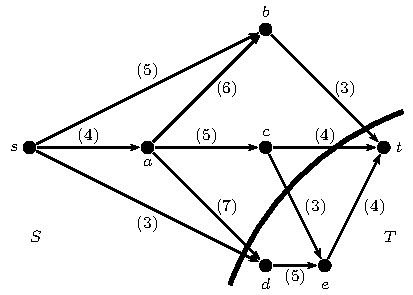
\includegraphics{fig11.pdf}
\end{center}
\end{frame}

\begin{frame}
 \frametitle{Ein weiteres Beispiel}
 Es seien $S = \big\{ s,c,d \big\}$ und $T = \big\{ a,b,e,t \big\}$. Dann gilt 
\[
\big(S,T\big) = \big\{ (s,a),(s,b), (c,e), (c,t), (d,e) \big\}.
\]
Dasselbe als Zeichnung:
\begin{center}
 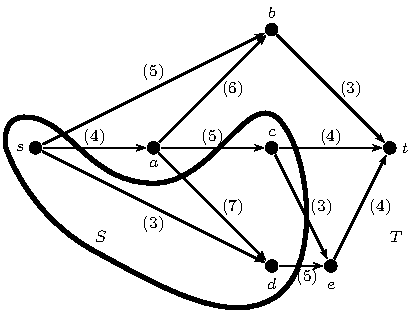
\includegraphics{fig12.pdf}
\end{center}
\end{frame}

\begin{frame}
 \frametitle{Ein drittes Beispiel}
 Es seien $S = \big\{ s \big\}$ und $T = \big\{ a,b,c,d,e,t \big\}$. Dann gilt 
\[
\big(S,T\big) = \big\{ (s,a), (s,b), (s,d) \big\}.
\]
Dasselbe als Zeichnung:
\begin{center}
 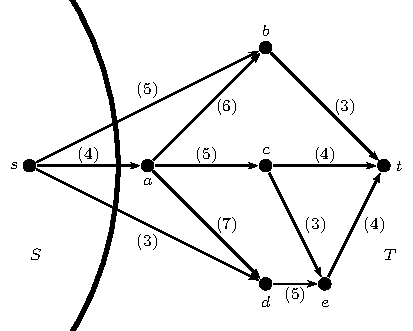
\includegraphics{fig13.pdf}
\end{center}
\end{frame}

\begin{frame}
\frametitle{Kapazität eines Schnitts}
Der Schnitt $(S,T)$ aus dem letzten Beispiel ist derjenige, der zur Schranke
\[
w(f) \leq 12
\]
für alle Flüsse $f$ auf $N$ geführt hat. \\ \vspace*{0.2cm}

In ähnlicher Weise führen alle Schnitte von $N$ zu einer oberen Schranke von $w(f)$; dies soll im Folgenden präzisiert werden. \\ \vspace*{0.2cm}

Zu diesem Zweck definieren wir, was die Kapazität eines Schnitts ist. \\ \vspace*{0.2cm}

\textbf{Definition:} Ist $(S,T)$ ein Schnitt von $N$, so wird die Zahl
\[
c(S,T) = \sum\limits_{e \in (S,T)}{c(e)}
\]
als \structure{Kapazität} von $(S,T)$ bezeichnet.
\end{frame}

\begin{frame}
\frametitle{Beispiele und Feststellung}
Die Kapazität eines Schnitts $(S,T)$ ist somit die Summe der Kapazitäten aller Kanten, die von $S$ ausgehen und nach $T$ führen. \\ \vspace*{0.2cm}

\textbf{Beispiele:} Es liege das Netzwerk von Folie 22 zugrunde und wir betrachten die obigen Beispiele für Schnitte $(S,T)$.
\begin{enumerate}[\bfseries 1.]
\item $S = \big\{ s,a,b,c \big\}$, $T = \big\{ d,e,t \big\}$: Dann gilt $c(S,T) = 3+7+3+4+3 = 20$.
\item $S = \big\{ s,c,d \big\}$, $T = \big\{ a,b,e,t \big\}$: Dann gilt $c(S,T) = 4+5+3+4+5 = 21$.
\item $S = \big\{ s \big\}$, $T = \big\{ a,b,c,d,e,t \big\}$: Dann gilt $c(S,T) = 4+5+3 = 12$.
\end{enumerate}
 \vspace*{0.2cm}
\textbf{Feststellung 2:} Ist $f$ ein beliebiger Fluss auf $N = (G,c,s,t)$ und ist $(S,T)$ ein beliebiger Schnitt, so gilt
\begin{equation}
\label{eq:9:1}
w(f) \leq c(S,T).
\end{equation}
\end{frame}

\begin{frame}
 \frametitle{Ein Hilfssatz}
 Diese Feststellung gibt die anschaulich einleuchtende Tatsache wieder, dass von $s$ nach $t$ niemals mehr fließen kann, als die Kapazität eines Schnitts zulässt. \\ \vspace*{0.2cm}

Zum Beweis von Feststellung 2 benötigen wir zunächst einen \alert{Hilfssatz, der auch noch an anderer Stelle nützlich sein wird}. Die Richtigkeit von Feststellung 2 wird sich -- wie wir unten sehen werden -- als unmittelbare Folgerung aus dem Hilfssatz ergeben. \\ \vspace*{0.2cm}

\textbf{Hilfssatz:}\label{page:9:4}
Ist $f$ ein Fluss auf $N = (G,c,s,t)$ mit $G=(V,E)$ und ist $S$ eine Teilmenge von $V$ mit $s \in S$ und $t \not\in S$, so gilt
\begin{equation}
\label{eq:9:2}
w(f) = f^+(S) - f^-(S).
\end{equation}
\end{frame}

\begin{frame}
 \frametitle{Minimale Schnitte}
 \textbf{Beweis von Feststellung 2:} Aufgrund des Hilfssatzes ergibt sich die Behauptung \eqref{eq:9:1} wie folgt:
\[
w(f) = f^+(S) - f^-(S) \leq f^+(S) = f(S,T) \leq c(S,T). \qquad \Box
\]\\
\vspace*{0.2cm}
\textbf{Definition:} Ein Schnitt $(S,T)$ von $N$ heißt \structure{minimal}, falls $c(S,T) \leq c(S',T')$ für alle Schnitte $(S',T')$ von $N$ gilt. \\ \vspace*{0.2cm}

Ist $f_0$ ein maximaler Fluss und $(S_0,T_0)$ ein minimaler Schnitt von $N$, so gilt nach Feststellung 2:
\begin{equation}
\label{eq:9:3}
w(f_0) \leq c(S_0,T_0).
\end{equation}
\end{frame}

\begin{frame}
 \frametitle{Max-Flow Min-Cut}
 Der folgende \alert{Satz von Ford und Fulkerson} aus dem Jahre 1956 besagt, dass in \eqref{eq:9:3} sogar Gleichheit gilt. \\ \vspace*{0.2cm}

\textbf{Satz (Max-Flow Min-Cut Theorem):} 
In einem Netzwerk ist der Wert eines maximalen Flusses immer gleich der Kapazität eines minimalen Schnittes. \\ \vspace*{0.2cm}

\textbf{Kurzfassung}: max-flow $=$ min-cut. \\ \vspace*{0.2cm}

Bevor wir den Satz beweisen, beschreiben wir eine \alert{Methode, mit der man einen gegebenen Fluss $f$ verbessern kann} -- vorausgesetzt natürlich, dass $f$ nicht bereits maximal ist. \\ \vspace*{0.2cm}

\alert{Diese Methode ist von zentraler Bedeutung}: Sie liefert nicht nur einen Beweis des Max-Flow Min-Cut Theorems, sondern ist auch die Grundlage für einen \alert{Algorithmus} zur Berechnung eines maximalen Flusses.
\end{frame}

\begin{frame}
 \frametitle{Beispiel einer Flussvergrößerung}
 \textbf{Beispiel:}\label{page:9:9} Für das Netzwerk von Folie 22 sei $f$ wie auf Folien 29/30 gegeben. Wir betrachten den (gerichteten) Pfad $(s,b,t)$, der die Quelle $s$ mit der Senke $t$ verbindet. Weder für die Kante $(s,b)$ noch für die Kante $(b,t)$ wird durch $f$ die Kapazität ausgeschöpft. Deshalb können wir in diesen beiden Kanten den Fluss soweit erhöhen, bis in einer der beiden Kanten die Kapazität erreicht ist. Dementsprechend definieren wir\footnote{Ist $(u,v)$ eine Kante, so müsste man streng genommen $f((u,v))$, $f_1((u,v))$, $c((u,v))$ etc. schreiben; der Einfachheit halber schreiben wir stattdessen immer $f(u,v)$, $f_1(u,v)$, $c(u,v)$ etc., was {\glqq}erlaubt{\grqq} und üblich ist, da Missverständnisse nicht möglich sind.}:
\begin{align*}
f_1(s,b) &= 2, \\
f_1(b,t) &= 3, \\
f_1(x,y) &= f(x,y) \text{ für alle anderen Kanten}.
\end{align*}
Da wir in beiden Kanten des Pfades $(s,b,t)$ den Fluss um den gleichen Betrag angehoben haben (nämlich um 1), ist $f_1$ wiederum ein Fluss\footnote{Man beachte: Eigenschaft 2) gilt nach wie vor.}:
\[
w(f_1) = w(f) + 1 = 7 + 1 = 8.
\]
\end{frame}

\begin{frame}
 \frametitle{Darstellung des verbesserten Flusses}
 Ersetzen wir in der Zeichnung von Folie 30 den alten Fluss $f$ durch den neuen Fluss $f_1$, so erhalten wir die folgende Darstellung:
 \begin{center}
  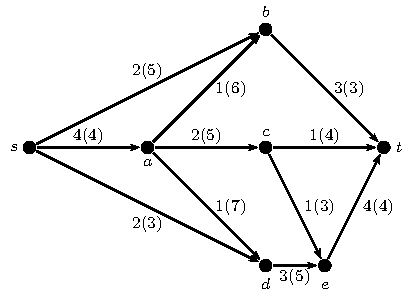
\includegraphics{fig14.pdf}
 \end{center}
\end{frame}

\begin{frame}
 \frametitle{Ein Pfad mit {\glqq}Rückwärtskanten{\grqq}}
 Wollen wir den Fluss weiter verbessern, so müssen wir etwas raffinierter vorgehen: 
\begin{quote}
{Wir durchlaufen Kanten \alert{auch in entgegengesetzter Richtung}.}
\end{quote}

\textbf{Genauer:} Wir betrachten die Folge
\begin{equation}
\label{eq:9:4}
(s,b,a,c,t)
\end{equation}
von Knoten. Längs dieser Folge bewegen wir uns in  unserem Netzwerk von $s$ nach $t$, wobei wir die Kante zwischen $a$ und $b$ rückwärts durchlaufen.
\end{frame}

\begin{frame}
 \frametitle{Definition des neuen Flusses}
 Man beachte: Für die {\glqq}Vorwärtskanten{\grqq} ist dabei die Kapazität nicht ausgeschöpft, und für die rückwärts durchlaufene Kante $e=(a,b)$ gilt $f_1(e) > 0$. \\ \vspace*{0.2cm}
 
 Wir definieren $f_2$ wie folgt:
\begin{align*}
f_2(s,b) &= f_1(s,b)+1, \\
f_2(a,b) &= f_1(a,b)-1, \\
f_2(a,c) &= f_1(a,c)+1, \\
f_2(c,t) &= f_1(c,t)+1, \\
\intertext{sowie}
f_2(x,y) &= f_1(x,y)
\end{align*}
für die übrigen Kanten. Es ergibt sich die folgende Darstellung von $f_2$:
\end{frame}

\begin{frame}
 \frametitle{Darstellung des neuen Flusses}
 \begin{center}
  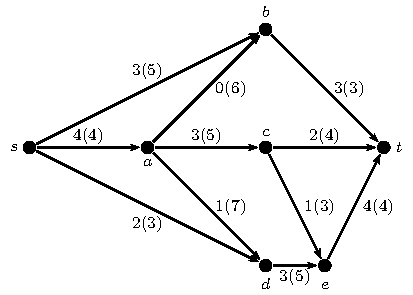
\includegraphics{fig15.pdf}
 \end{center}

\end{frame}

\begin{frame}
 \frametitle{$f_2$ ist ein verbesserter Fluss}
 Da wir für alle {\glqq}Vorwärtskanten{\grqq} den Fluss um denselben Betrag erhöht haben und gleichzeitig für alle {\glqq}Rückwärtskanten{\grqq} den Fluss um genau diesen Betrag erniedrigt haben (ohne die Kapazitäten zu überschreiten bzw. $0$ zu unterschreiten), ist $f_2$ wiederum ein Fluss\footnote{Man beachte: Eigenschaft 2) gilt nach wie vor.}. Es gilt
\[
w(f_2) = w(f_1) + 1 = 8+1 = 9.
\]
\end{frame}

\begin{frame}
 \frametitle{Eine weitere Verbesserung}
 In ähnlicher Weise können wir den Fluss $f_2$ verbessern: Diesmal benutzen wir die Knotenfolge
\begin{equation}
\label{eq:9:5}
(s,d,e,c,t)
\end{equation}
und erhalten ganz entsprechend einen verbesserten Fluss $f_3$, für den $w(f_3)=10$ gilt:
\begin{center}
  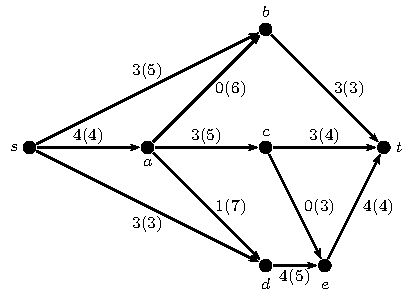
\includegraphics{fig16.pdf}
 \end{center}
\end{frame}

\begin{frame}
 \frametitle{Ein Beleg für die Optimalität von $f_3$}
 Nun können wir keine Knotenfolge mehr finden, die wie die Folgen \eqref{eq:9:4} und \eqref{eq:9:5} geeignet wäre, den Fluss $f_3$ zu verbessern. Wir haben daher den \alert{Verdacht}, dass $f_3$ ein maximaler Fluss ist. \\ \vspace*{0.2cm}

\textbf{Frage:} Wie können wir diesen Verdacht in eine Gewissheit verwandeln? \\ \vspace*{0.2cm}

\textbf{Antwort:} Unser Verdacht wird Gewissheit, wenn wir einen \alert{Beleg (Zertifikat)} für die Optimalität von $f_3$ vorlegen. \\ \vspace*{0.2cm}

\alert{Hier ist der gewünschte Beleg:} Der Schnitt $(S,T)$ mit $S= \big\{ s,b \big\}$ und $T = \big\{ a,c,d,e,t \big\}$ ist ein Zertifikat für die Optimalität von $f_3$, da für diesen Schnitt $c(S,T)=10$ gilt. Da ebenfalls $w(f_3)=10$ gilt, wissen wir (vgl. \eqref{eq:9:1}): Einen besseren Fluss kann es nicht geben.
\end{frame}

\begin{frame}
 \frametitle{Flussvergrößerungen}
 Im vorangegangenen Beispiel gab es drei Flussvergrößerungen: Beim Übergang zu $f_1$ kam zunächst die Knotenfolge $(s,b,t)$ zum Einsatz, anschließend wurden die Knotenfolgen \eqref{eq:9:4} und \eqref{eq:9:5} verwendet. Derartige Knotenfolgen werden \structure{flussvergrößernde Pfade} genannt. \\ \vspace*{0.2cm}
 
 Bevor wir diesen Begriff zusammen mit verwandten Begriffen definieren, seien \alert{zwei Bemerkungen} vorausgeschickt:
\begin{enumerate}[\bfseries 1.]
	\item Wenn eine Rückwärtskante in einem flussvergrößernden Pfad $P$ vorkommt, so handelt es sich bei $P$ nicht um einen Pfad im gerichteten Graphen $G=(V,E)$. (Pfade im üblichen Sinne enthalten keine Rückwärtskanten.) Es ist trotzdem üblich, von einem Pfad zu sprechen, denn: Die Knotenfolge von $P$ beschreibt einen Pfad \alert{im $G$ zugrundeliegenden ungerichteten Graphen}. Dasselbe kurz und knapp gesagt: \alert{$P$ ist ein Pfad, wenn man die Kantenrichtungen ignoriert}.
\end{enumerate}
\end{frame}

\begin{frame}
 \frametitle{Antiparallele Kanten}
 Die zweite Bemerkung hat mit der Tatsache zu tun, dass in $G$ Paare von \structure{antiparallelen Kanten} zugelassen sind: Es könnte, wie in der nachfolgenden Figur, neben der Kante $(a,b)$ auch die Kante $(b,a)$ in $G$ vorkommen.\\ \vspace*{0.2cm}
 \begin{center}
  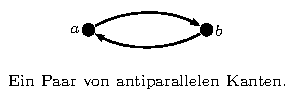
\includegraphics{fig17.pdf}
 \end{center}
\end{frame}

\begin{frame}
 \frametitle{Zweite Bemerkung}
 \begin{enumerate}[\bfseries 1.]
  \addtocounter{enumi}{1}
	\item Da in $G$ antiparallele Kanten vorkommen können, werden wir gelegentlich nicht nur die Knoten eines flussvergrößernden Pfades $P$ angeben, \alert{sondern zusätzlich auch die Kanten von $P$.} Dies wird zum Beispiel weiter unten in \eqref{eq:9:6} so gemacht und dient der \alert{Klarheit und Eindeutigkeit}: Falls es zwei Möglichkeiten gibt, soll eindeutig feststehen, welche Kante zu $P$ gehört und welche nicht.
\end{enumerate}
\end{frame}

\begin{frame}
 \frametitle{Voraussetzungen}
 Zunächst die \alert{Voraussetzungen für die folgende \textbf{Definition:}} Gegeben sei ein Netzwerk $N=(G,c,s,t)$ mit $G=(V,E)$ sowie ein Fluss $f$ auf $N$; $k\geq 1$ sei eine ganze Zahl. Wir betrachten die Folge
	\begin{equation}
	\label{eq:9:6}
	P: s = v_1,e_1,\ldots,e_{k-1},v_k,
	\end{equation}
	die in $s$ beginnt aber nicht unbedingt in $t$ endet. Auf $P$ wechseln sich Knoten und Kanten ab. \\ \vspace*{0.2cm}
	
	\textbf{Genauer:} Es gilt $v_i \in V$ ($i=1,\ldots,k$) und $e_i \in E$ ($i=1,\ldots,k-1$). Außerdem soll es in $P$ \alert{keine Knotenwiederholungen} geben.
\end{frame}

\begin{frame}
 \frametitle{Eine zentrale Definition}
 \textbf{Definition:}
 \begin{enumerate}[a)]
		\item Eine solche Folge $P$ nennt man einen \structure{flussvergrößernden} oder \structure{zunehmenden Pfad}, falls $v_k=t$ gilt und falls für jedes $i \in \big\{ 1,\ldots,k-1 \big\}$ entweder
		\begin{equation}
		\label{eq:9:7}
		e_i = (v_i,v_{i+1}) \quad\text{und}\quad f(v_i,v_{i+1}) < c(v_i, v_{i+1})
		\end{equation}
		oder
		\begin{equation}
		\label{eq:9:8}
		e_i = (v_{i+1}, v_i) \quad\text{und}\quad 0 < f(v_{i+1}, v_i)
		\end{equation} 
		erfüllt ist.
		
		\item Wir werden auch den Fall betrachten, dass $P$ alle unter a) genannten Bedingungen erfüllt, nur $v_k=t$ gilt möglicherweise nicht. Dann sprechen wir von einem \structure{zunehmenden Pfad nach $v_k$}. \label{page:9:7}
		
		\item Gilt \eqref{eq:9:7}, so wird $e_i$ \structure{Vorwärtskante} von $P$ genannt; gilt \eqref{eq:9:8}, so heißt $e_i$ \structure{Rückwärtskante} von $P$.
	\end{enumerate}
 \textbf{Weitere Sprechweisen:} Unter den Voraussetzungen der obigen Definition sagen wir auch \structure{$f$-vergrößernder Pfad} anstelle von flussvergrößernder Pfad. 
\end{frame}

\begin{frame}
 \frametitle{Ein Beispiel}
 Wir betrachten das folgende \textbf{Beispiel:}
 \begin{center}
  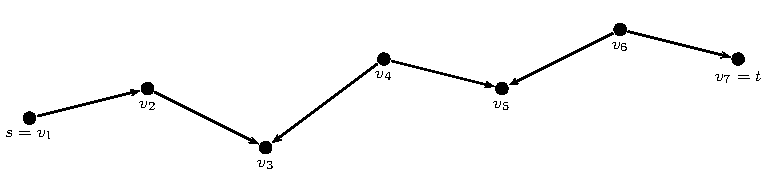
\includegraphics[width=0.9\textwidth]{fig18.pdf}
 \end{center}
 Die Vorwärtskanten in diesem Beispiel sind $(v_1,v_2)$, $(v_2,v_3)$, $(v_4,v_5)$, $(v_6,v_7)$ und die Rückwärtskanten sind $(v_4,v_3)$ und $(v_6,v_5)$. Soll dies ein flussvergrößernder Pfad sein, so muss also gelten:
\begin{align*}
f(v_1,v_2) &< c(v_1,v_2), \\
f(v_2,v_3) &< c(v_2,v_3), \\
f(v_4,v_3) &> 0, \\
f(v_4,v_5) &< c(v_4,v_5), \\
f(v_6,v_5) &> 0, \\
f(v_6,v_7) &< c(v_6,v_7).
\end{align*}
\end{frame}

\end{document}
